% =============================================================================
% Draft mục 3.3.6 — Execution Engine (Orchestrator + BridgeService)
% =============================================================================

\subsection{Execution Engine: Orchestrator và BridgeService}
\label{sec:execution-engine}

Khi Matching Engine sản sinh một \texttt{MatchResult} chứa các chu
trình đã được khớp về mặt logic, công việc còn lại là biến chu trình
đó thành các giao dịch trên chuỗi sao cho \emph{tài sản chỉ thực sự
chuyển nếu mọi nhánh trong chu trình đều thành công}. Đây là vai trò
của Execution Engine, được tách thành hai tầng: \textbf{Orchestrator}
chịu trách nhiệm lập kế hoạch và điều phối, và \textbf{BridgeService}
là tầng thấp gói gọn các tương tác cụ thể với hợp đồng HTLC trên từng
chuỗi.

\subsubsection*{Mô hình "presiding/responding"}

Một chu trình có thể chứa nhiều cạnh trên cùng một chuỗi (nhiều
intent có cùng chuỗi nguồn nhưng khác chuỗi đích, hoặc ngược lại).
Với HTLC chuẩn, mỗi cạnh sẽ là một giao dịch riêng — chi phí gas
cao và phải đồng bộ nhiều secret/hashlock. OceanLink tận dụng tính
chất multi-fill của HTLC (xem
\S\ref{sec:smart-contract-layer}) để \emph{gom} các cạnh cùng chuỗi
nguồn vào \emph{một} order với nhiều fill, giảm số giao dịch
cần phát.

Trong mỗi \texttt{MatchResult}, một order consolidated được Orchestrator
chọn làm \emph{order chủ tịch} (\texttt{presiding order}); các order
còn lại là \emph{order phản hồi} (\texttt{responding orders}).
Phân vai này quyết định ai sinh bí mật:

\begin{itemize}
  \item \textbf{Order chủ tịch} sinh các bí mật $s_i$ tươi (random
    256-bit) tại lúc tạo, và publish các hashlock
    $h_i = \mathrm{SHA256}(s_i)$ qua sự kiện \texttt{FillCreated}.
  \item \textbf{Các order phản hồi} \emph{không sinh bí mật mới}; thay
    vào đó, chúng tái sử dụng các $h_i$ đã có. Mỗi fill trong order
    phản hồi liên kết với đúng một fill trong order chủ tịch (qua
    chỉ số chu trình), do đó cùng chia sẻ một preimage.
\end{itemize}

Cấu trúc này là cốt lõi của tính nguyên tử: \emph{biết một preimage
$s_i$ là điều kiện đủ để mở khoá tất cả các fill chia sẻ
$h_i$ trên mọi chuỗi}. Khi order chủ tịch được rút bằng $s_i$, giá
trị $s_i$ trở thành công khai trên chuỗi — bất kỳ ai (Orchestrator
trong trường hợp này) cũng có thể dùng nó để rút các fill phản hồi
tương ứng trên các chuỗi khác.

\subsubsection*{Thuật toán \texttt{handleMatchResults}}

Orchestrator nhận một mảng \texttt{MatchResult} từ scheduler. Với
mỗi \texttt{MatchResult} (xử lý tuần tự để giữ thứ tự thời gian
matchId), thực hiện các bước sau:

\begin{enumerate}
  \item Đặt \texttt{ExecutionRecord} cho \texttt{matchId} sang
    \texttt{pending} và persist vào bảng \texttt{executions}.
  \item Trích các \emph{send action} từ chu trình
    (\texttt{extractSendActionsFromCycles}). Mỗi send action mô tả:
    cạnh nào, chuỗi nguồn nào, người gửi nào (địa chỉ ví), người
    nhận nào, số tiền bao nhiêu, thuộc chu trình nào.
  \item Gom các action có cùng \emph{chuỗi nguồn + người gửi} thành
    nhóm (\texttt{groupActionsByChainKey}); mỗi nhóm sẽ trở thành
    \emph{một} order multi-fill trên chuỗi đó.
  \item Chọn nhóm đầu tiên làm presiding, gọi
    \texttt{executePresidingOrder} $\rightarrow$ BridgeService.\texttt{createOrder}
    với cờ \texttt{isPresiding=true}. Kết quả: orderId trên chuỗi,
    txHash, danh sách $\{s_i, h_i\}$ cho các fill.
  \item Dựng map \emph{cycleIdx $\rightarrow$ hashlock} từ kết quả presiding để
    các order phản hồi biết phải tái sử dụng hashlock nào cho mỗi
    chu trình.
  \item Gọi \texttt{executeNonPresidingOrders} cho từng nhóm còn lại,
    truyền kèm map hashlock; mỗi nhóm tạo một order phản hồi với
    \texttt{isPresiding=false}, không sinh secret mới.
  \item Sau khi mọi HTLC đã có mặt trên chuỗi: gọi
    \texttt{verifyAndWithdrawOrders}. Bước này thực hiện các giao
    dịch \texttt{withdraw} với preimage tương ứng — trên cả chuỗi
    chủ tịch và các chuỗi phản hồi — để đưa tài sản về tay người
    nhận thực sự.
  \item Persist \texttt{ExecutionRecord} với \texttt{status="done"}
    và đầy đủ dữ liệu (presiding order info, danh sách responding
    withdraws, các secret từng fill) vào bảng \texttt{executions}.
  \item Phát các sự kiện lifecycle qua \texttt{orderEvents}:
    \texttt{plan}, \texttt{htlc\_created} (cho mỗi nhóm),
    \texttt{withdrawn}, \texttt{done}.
\end{enumerate}

Nếu bất kỳ bước nào throw, khối catch đặt \texttt{ExecutionRecord}
sang \texttt{status="error"} với thông điệp lỗi tương ứng và phát
sự kiện \texttt{error}. \emph{Không có rollback on-chain}: các HTLC
đã được tạo sẽ tự hoàn lại sau \texttt{timelock} hết hạn (cơ chế
refund của hợp đồng — xem \S\ref{sec:smart-contract-layer}).

\subsubsection*{Phân tích tính nguyên tử (atomicity)}

Hệ thống đảm bảo \emph{không có trạng thái} mà một bên nhận tài sản
trong khi bên đối ứng mất tài sản. Phân tích bốn pha có thể xảy ra
sai sót:

\begin{itemize}
  \item \textbf{Sai sót khi tạo presiding.} Nếu giao dịch
    \texttt{newOrder} của presiding fail, không có HTLC nào được
    tạo, không có tài sản nào bị khoá; thoát an toàn.
  \item \textbf{Sai sót khi tạo responding.} Nếu một responding order
    fail sau khi presiding đã có mặt trên chuỗi, presiding sẽ ở
    trạng thái khoá nhưng không ai rút (vì bên đối ứng không có HTLC
    để rút). Sau \texttt{timelock} (mặc định 10 phút), người gửi
    presiding gọi \texttt{refund} để lấy lại; bên đối ứng cũng không
    chịu thiệt hại nào vì chưa khoá tài sản.
  \item \textbf{Sai sót khi withdraw presiding.} Nếu withdraw fail
    sau khi mọi HTLC đã được tạo, các HTLC sẽ bị refund sau
    timelock — như trường hợp trên.
  \item \textbf{Sai sót khi withdraw responding.} Đây là tình huống
    tinh tế nhất: presiding đã được rút (bí mật $s_i$ đã công khai
    trên chuỗi), nhưng Orchestrator không kịp gọi withdraw cho
    responding. Trong trường hợp này, \emph{bất kỳ ai} (không chỉ
    Orchestrator) cũng có thể đọc $s_i$ từ event
    \texttt{FillWithdrawn} của chuỗi presiding và gọi withdraw cho
    fill responding tương ứng. Hợp đồng cho phép địa chỉ admin (nếu
    được whitelist) thực hiện thay người nhận — kết hợp với cờ
    \texttt{allowWithdrawAfterExpiry} (đặt \texttt{true} khi deploy)
    cho phép cứu các fill ngay cả sau khi timelock đã hết.
\end{itemize}

\subsubsection*{BridgeService: tầng tương tác với chuỗi}

\texttt{BridgeService} là một wrapper mỏng xung quanh viem (thư viện
TypeScript cho EVM), cung cấp các phép nguyên thủy:

\begin{itemize}
  \item \texttt{createOrder(\{ receivers, amounts, chain, isPresiding,
    onBehalfOf \})} — gọi hàm \texttt{newOrder} của hợp đồng HTLC.
    Khi \texttt{isPresiding=true}, sinh secret tươi và tính hashlock;
    khi \texttt{false}, nhận hashlock từ Orchestrator. Tham số
    \texttt{onBehalfOf} cho phép admin tạo order thay mặt một ví
    người dùng khác (xem mục về cờ admin trong
    \S\ref{sec:smart-contract-layer}).
  \item \texttt{withdraw(\{ orderId, fillId, preimage, chain \})} —
    gọi \texttt{withdraw} trên hợp đồng tương ứng.
  \item \texttt{refund(\{ orderId, chain \})} — gọi \texttt{refund} —
    chủ yếu được kích hoạt thủ công hoặc bởi một tiến trình
    "garbage collector" sau khi timelock hết hạn (chưa nằm trong
    scope của MVP).
  \item \texttt{approve(...)} — pre-approve USDC cho hợp đồng HTLC.
\end{itemize}

BridgeService dùng \emph{một signer cho mỗi chuỗi}, ánh xạ qua biến
môi trường: ví LP $B$ ký giao dịch trên Ethereum Sepolia, $C$ trên
Base Sepolia, $D$ trên Arbitrum Sepolia. Đối với các giao dịch read
(estimate gas, balanceOf, allowance), BridgeService dùng signer
\texttt{PRIVATE\_KEY\_ADMIN} dưới vai trò "ambient reader".

\subsubsection*{Vai trò trong sơ đồ tổng thể}

Execution Engine là \emph{ranh giới on-chain duy nhất} của hệ thống.
Mọi giao dịch đi từ off-chain xuống on-chain đều phải qua
BridgeService; Orchestrator không bao giờ tự gọi viem mà phải đi
qua wrapper. Phân chia này có hai lợi ích:

\begin{itemize}
  \item \emph{Test-friendly}: trong test, BridgeService có thể được
    thay bằng một fake để Orchestrator chạy không cần kết nối
    chain, giữ cho unit test của logic điều phối nhanh và ổn định.
  \item \emph{Single point of change} cho việc mở rộng sang chuỗi
    mới: thêm một chuỗi (vd. Avalanche) chỉ yêu cầu thêm cấu hình
    trong \texttt{config/chains.ts} và một signer cho ví tương ứng;
    Orchestrator không phải sửa.
\end{itemize}

% -----------------------------------------------------------------------------
% Mô hình thực thi ba lớp — chuyển từ section riêng vào đây vì Execution
% Engine là điểm điều phối chiến lược thực thi của một intent.
% -----------------------------------------------------------------------------

\subsubsection*{Mô hình thực thi ba lớp}
\label{sec:three-layer-model}

Như đã đề cập ở phần dẫn nhập của chương, OceanLink không cố ép mọi
intent qua một con đường thanh toán duy nhất mà tổ chức việc thanh
toán thành \emph{ba lớp thực thi} áp dụng tuần tự. Execution Engine
là thành phần điều phối hai trong ba lớp này (Lớp 1 và Lớp 2 — cả hai
đều settle qua HTLC do BridgeService phát) và bàn giao Lớp 3 cho
Fallback Bridge Aggregator (xem \S\ref{sec:fallback-bridge}). Việc
trình bày mô hình ở đây — bên trong tiểu mục Execution Engine — phản
ánh đúng vị trí của thành phần này như một \emph{strategy router}
giữa các lớp.

\paragraph{Lớp 1 --- Netting Layer.} \emph{Mục tiêu}: thanh toán bằng
cách bù trừ trực tiếp các intent đối ứng, không cần thanh khoản
ngoài. \emph{Cơ chế}: Matching Engine
(\S\ref{sec:matching-engine}) mô hình hoá tập intent đang chờ thành
đồ thị có hướng và tìm các chu trình bù trừ; mỗi chu trình thoả
ngưỡng chấp nhận sẽ được Orchestrator + BridgeService thanh toán
nguyên tử qua HTLC trên các chuỗi liên quan, đúng theo mô hình
presiding/responding ở phần đầu tiểu mục này. \emph{Ưu điểm}: chi
phí gần bằng không (chỉ phí gas), trust-minimized vì không cần
solver, chất lượng thực thi tối ưu (không trượt giá). \emph{Nhược
điểm}: phụ thuộc vào sự xuất hiện của intent đối ứng — có thể phải
chờ nhiều tick trước khi tìm được match.

\paragraph{Lớp 2 --- Intent Accelerator Layer.} \emph{Mục tiêu}:
thanh toán nhanh phần intent không match được trong Lớp 1, bằng
cách cho phép người dùng đính kèm \emph{incentive fee} để các solver
bên ngoài cạnh tranh fill và hưởng phần fee này. \emph{Cơ chế}: phần
dư của intent được broadcast đến các solver đã đăng ký; mỗi solver
đề xuất một mức giá riêng, người gửi chấp nhận quote tốt nhất. Một
biến thể quan trọng là \emph{incentive Dutch auction}: phí thưởng
cho solver bắt đầu bằng không và tăng dần theo thời gian, tạo trò
chơi chiến lược giữa "thực thi sớm với phần thưởng thấp" và "chờ
phần thưởng cao hơn nhưng đối mặt rủi ro mất lượt". Khi solver
commit, kênh thanh toán cuối vẫn là HTLC do BridgeService phát ---
khác Lớp 1 ở \emph{nguồn thanh khoản} (solver bên ngoài thay vì
intent nội bộ), không khác ở \emph{cơ chế settle}. \emph{Ưu điểm}:
tốc độ thực thi gần như tức thời. \emph{Nhược điểm}: chi phí cao
hơn Lớp 1 (incentive trả cho solver), tiềm năng các hành vi chiến
lược như selective fill.

\paragraph{Lớp 3 --- Fallback Bridge Aggregator.} \emph{Mục tiêu}:
bảo đảm completion cho intent vẫn còn dư sau hai lớp trên, bằng
cách định tuyến qua một bridge bên thứ ba có thanh khoản thực sự.
Lớp này \emph{bỏ qua HTLC} và đi qua kênh thanh toán riêng của
bridge — Execution Engine chỉ tham gia đến bước "đánh dấu intent
chuyển sang Lớp 3" rồi bàn giao điều phối cho Fallback Bridge
Aggregator (\S\ref{sec:fallback-bridge}). \emph{Ưu điểm}: hoàn tất
gần như chắc chắn. \emph{Nhược điểm}: chi phí cao nhất, độ trễ phụ
thuộc bridge bên ngoài.

\paragraph{Vòng đời một intent qua ba lớp.}

\begin{enumerate}
  \item Intent được \texttt{validateIntent} ở API Gateway và đưa vào
    OrderStore với trạng thái \texttt{QUEUED}.
  \item Trong cửa sổ thời gian $T_{\text{net}}$, Matching Engine cố
    tìm cycle ở mỗi tick:
    \begin{itemize}
      \item Nếu tìm được cycle khớp toàn bộ: trạng thái chuyển
        \texttt{MATCHED}, Execution Engine settle nguyên tử qua
        HTLC, intent kết thúc ở Lớp 1.
      \item Nếu khớp một phần: phần khớp được settle, phần dư trở
        thành \texttt{PARTIAL} và tiếp tục chờ.
    \end{itemize}
  \item Khi cửa sổ $T_{\text{net}}$ trôi qua mà phần dư vẫn còn,
    intent (hoặc phần dư của nó) được chuyển sang Lớp 2: broadcast
    cho solver, chạy Dutch auction. Nếu một solver commit, phần đó
    được settle qua cùng kênh HTLC; nếu không, sang Lớp 3.
  \item Lớp 3 chọn bridge tốt nhất, phát giao dịch qua adapter và
    theo dõi đến khi hoàn tất hoặc thất bại. Đây là điểm cuối ---
    không có Lớp 4.
\end{enumerate}

Trật tự "leo dần" này đảm bảo phần lớn intent hưởng chi phí thấp
nhất có thể (Lớp 1), một số ít chấp nhận trade-off cho tốc độ (Lớp
2), và \emph{không có intent nào bị treo vô thời hạn} (Lớp 3 luôn
sẵn sàng làm điểm thoát).

\begin{figure}[H]
  \centering
  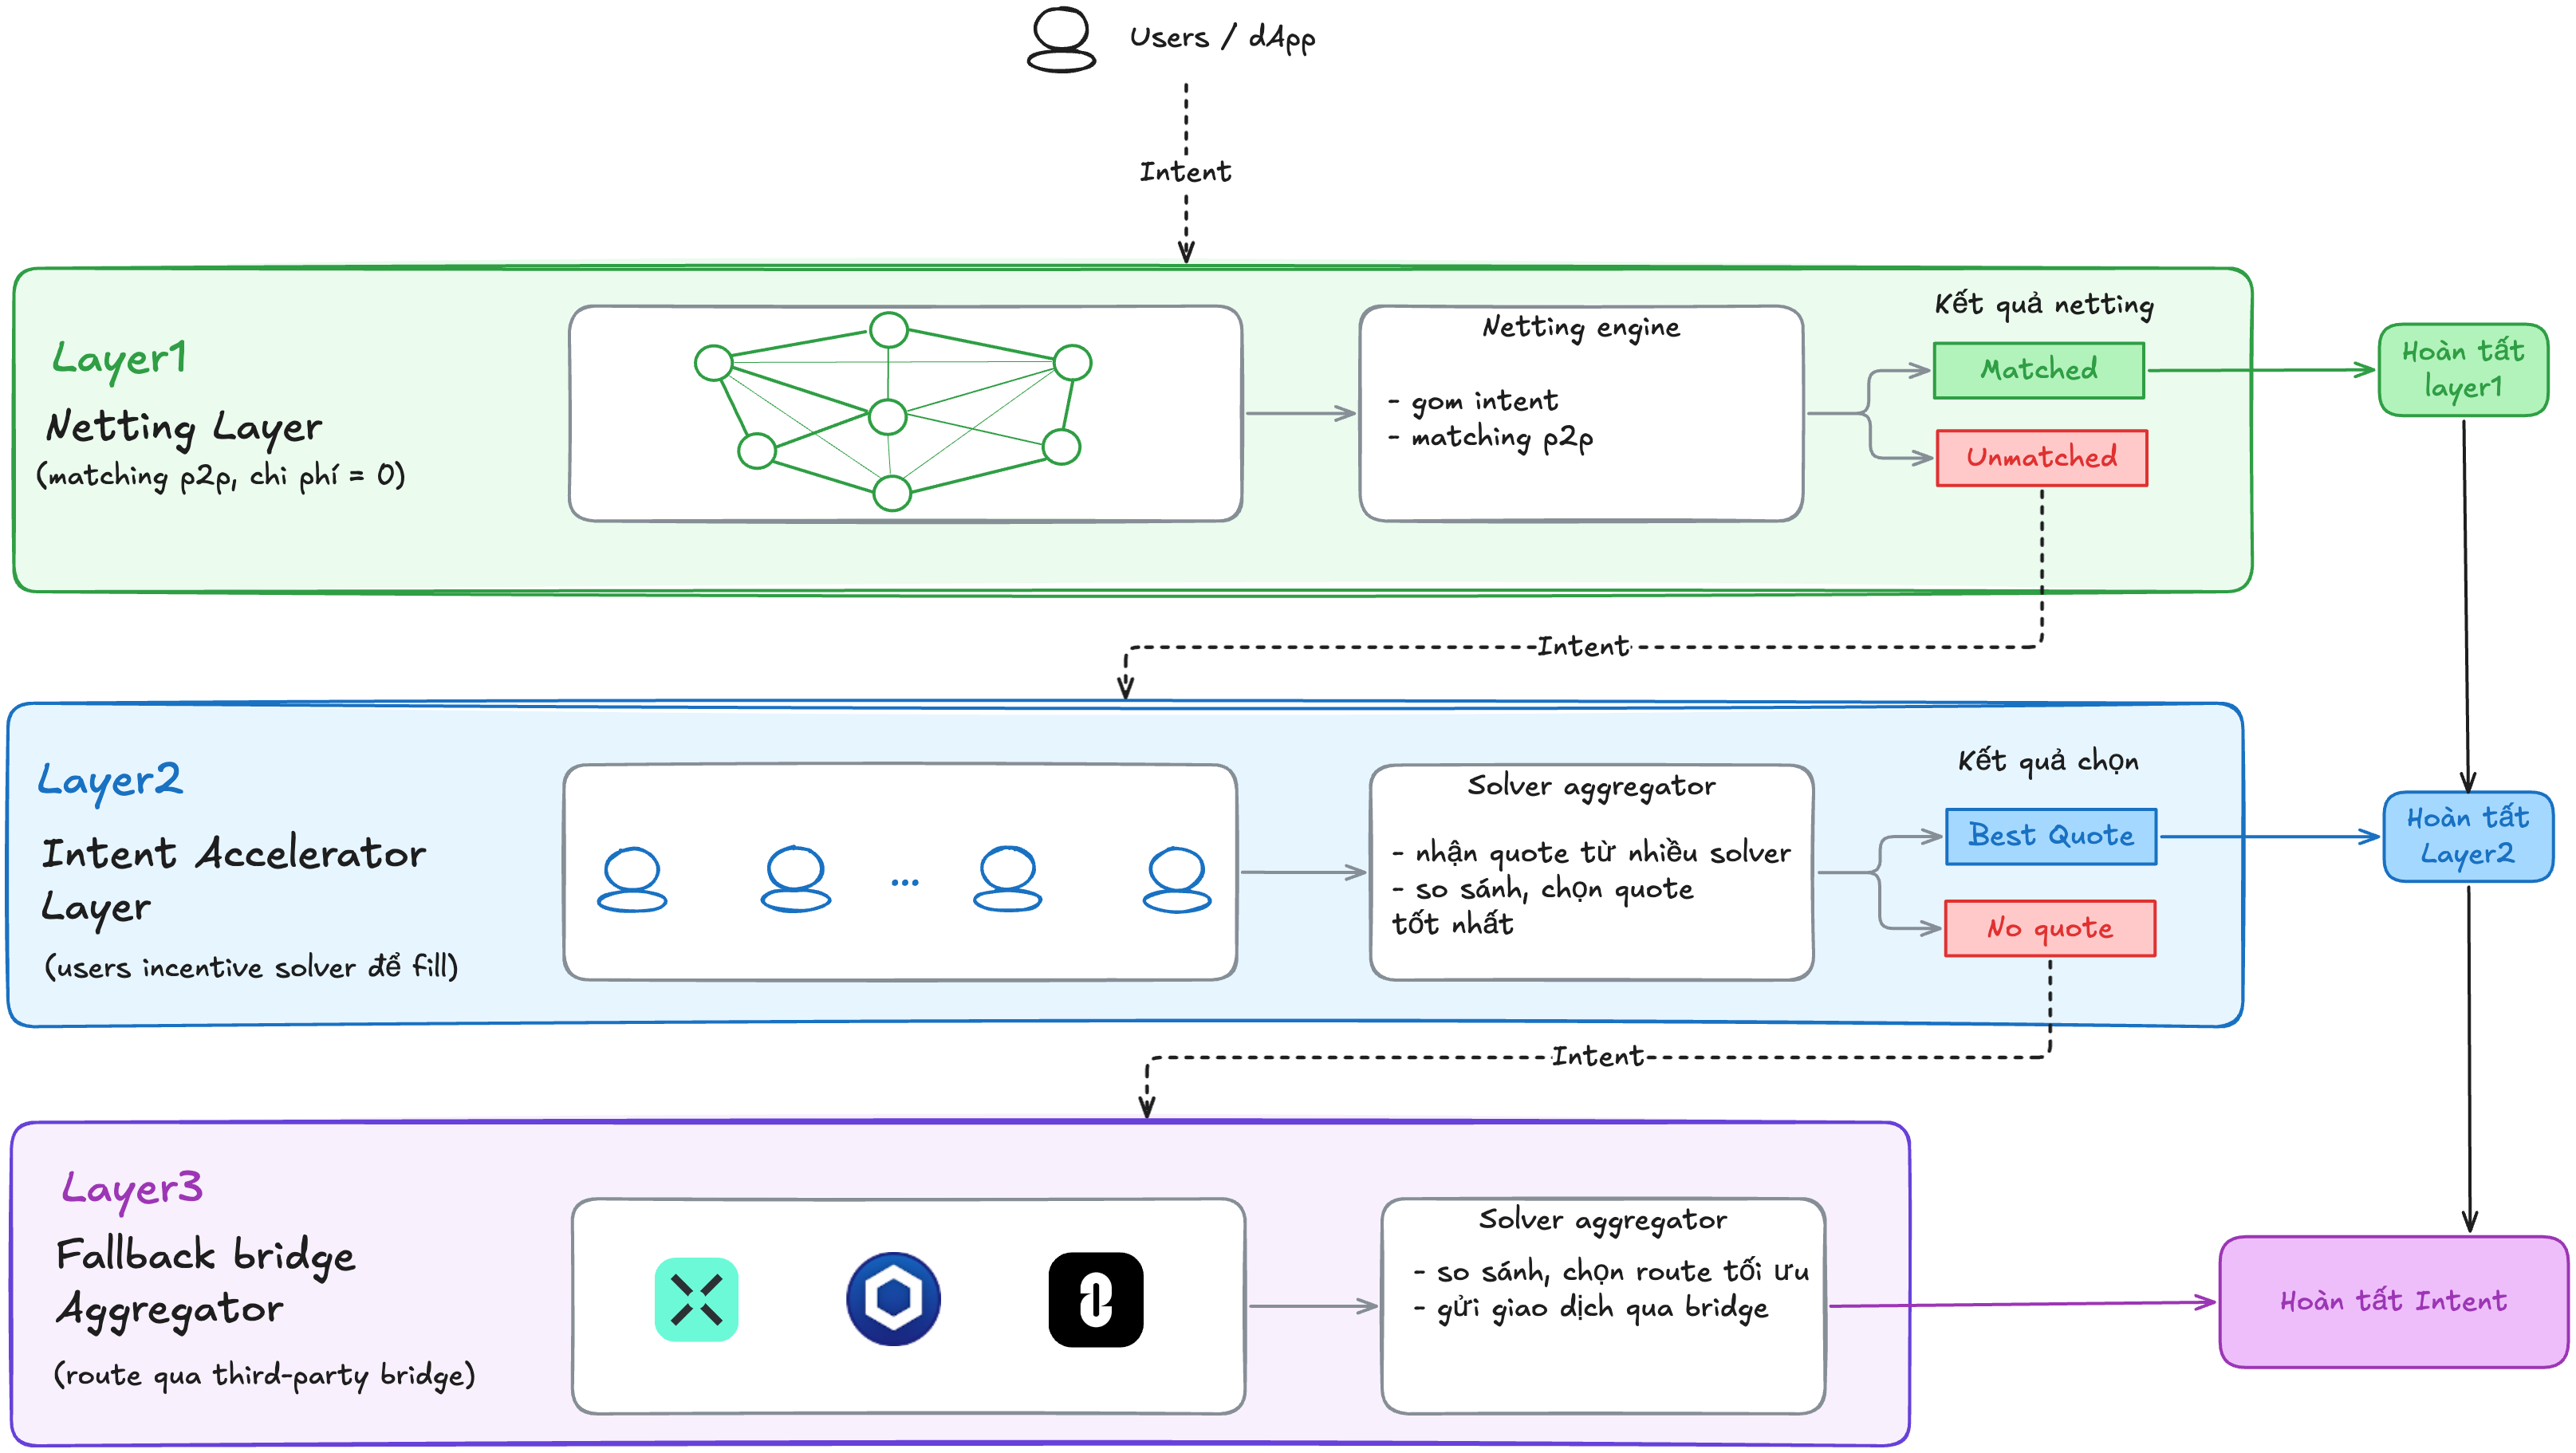
\includegraphics[width=\linewidth]{figures/c3/intent-layer}
  \caption{Vòng đời của một intent qua ba lớp thực thi: bắt đầu ở
  Netting Layer, leo dần xuống Intent Accelerator Layer khi không
  tìm được đối tác bù trừ, và cuối cùng được định tuyến qua
  Fallback Bridge Aggregator nếu cần.}
  \label{fig:intent-lifecycle}
\end{figure}

\paragraph{Ánh xạ các lớp vào thành phần.} Mặc dù ba lớp khác nhau
ở \emph{nguồn thanh khoản} và \emph{cơ chế tìm đối tác}, chúng dùng
chung phần lớn các thành phần đã giới thiệu:

\begin{itemize}
  \item \textbf{Lớp 1} dùng API Gateway, OrderStore, Matching Engine
    (MatchScheduler + MatchingService + Solver), Execution Engine và
    Smart Contract Layer (HTLC).
  \item \textbf{Lớp 2} dùng cùng API Gateway và OrderStore, nhưng
    thay Matching Engine bằng một bộ phát quote tới các solver bên
    ngoài; Execution Engine và HTLC vẫn là kênh thanh toán cuối.
  \item \textbf{Lớp 3} dùng Fallback Bridge Aggregator để chọn và
    gọi adapter bridge phù hợp; bỏ qua HTLC và đi qua kênh thanh
    toán riêng của bridge bên thứ ba.
\end{itemize}

\paragraph{Phạm vi triển khai trong luận văn.}

\begin{itemize}
  \item \textbf{Lớp 1} đã được cài đặt đầy đủ: matching engine, HTLC
    multi-fill, orchestrator. Đây là phần tập
    trung của các tiểu mục thiết kế chi tiết và phần đo benchmark
    trong chương Đánh giá.
  \item \textbf{Lớp 2} được trình bày ở mức thiết kế: interface,
    Dutch auction incentive, lưu đồ tương tác. Cài đặt cụ thể nằm
    ngoài scope.
  \item \textbf{Lớp 3} được trình bày ở mức thiết kế: interface
    \texttt{BridgeAdapter} và danh sách bridge ứng cử
    (\S\ref{sec:fallback-bridge}). Cài đặt cụ thể nằm ngoài scope.
\end{itemize}

Phần Future Work (chương cuối) liệt kê các hạng mục cần hoàn thiện
để Lớp 2 và Lớp 3 đi vào hoạt động đầy đủ.
